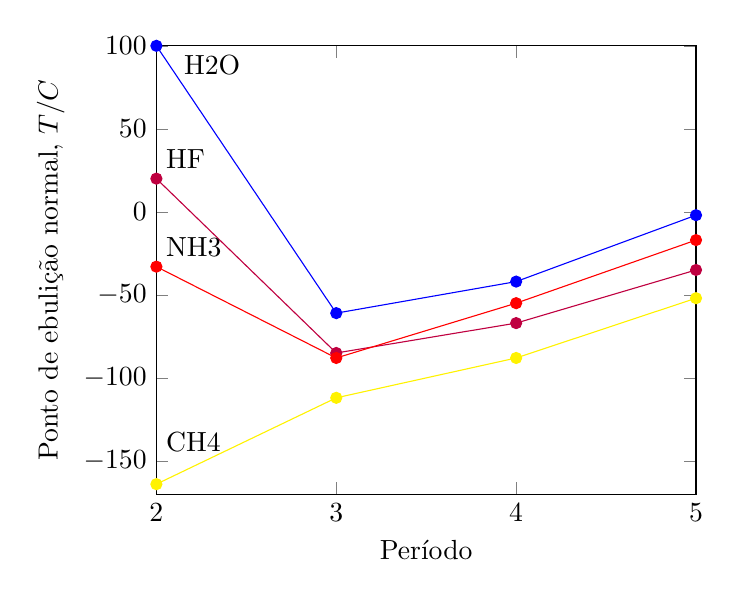
\begin{tikzpicture}
    \begin{axis}
    [
        grid = none,
        ylabel = {Ponto de ebulição normal, $T/\unit{\degree C}$},
        xlabel = {Período},
        ymin=-170, ymax=100,
        xmin=2, xmax=5,
        xtick = {2, 3, 4, 5},
    ]    
    %% GRUPO 17
    \addplot [ mark=*, color=purple ] coordinates
        { 
            (2,  20)
            (3, -85)
            (4, -67)
            (5, -35)
        };
    \node [anchor = south west] at (axis cs: 2, 20) { \ce{HF} };

    %% GRUPO 16
    \addplot [ mark=*, color=blue ] coordinates
        { 
            (2, 100)
            (3, -61)
            (4, -42)
            (5,  -2)
        };
    \node [anchor = north west] at (axis cs: 2.1, 100) { \ce{H2O} };

        %% GRUPO 15
    \addplot [ mark=*, color=red ] coordinates
        { 
            (2, -33)
            (3, -88)
            (4, -55)
            (5, -17)
        };
    \node [anchor = south west] at (axis cs: 2, -33) { \ce{NH3} };

    %% GRUPO 14
    \addplot [ mark=*, color=yellow ] coordinates
        { 
            (2, -164)
            (3, -112)
            (4,  -88)
            (5,  -52)
        };
    \node [anchor = south west] at (axis cs: 2, -150) { \ce{CH4} };
    \end{axis}
\end{tikzpicture}
